\section{Introduction}

\textit{April 27th, 2010 - Philadelphia Convention Center (Main Hall):}  The robot handlers Daniel M. Lofaro 
and Robert Ellenberg were preparing the adult-size humanoid robot Jaemi Hubo\footnote{Jaemi Hubo Home Page: http://dasl.mem.drexel.edu/HUBO} at an outreach demonstration for the 
\textit{Arts \& Science Council} of Philadelphia.  During the dress rehearsal one of Jaemi's actuators failed 
during a demonstration of active balancing and she fell off of a 4 foot high stage.  The results of the impact 
can be found in Fig.~\ref{fig:fall} and on YouTube\footnote{Jaemi Hubo Fall: http://www.youtube.com/watch?v=DF8zAM4FLB4\label{link:fall}}.  
This annual event was a high profile fund raiser for the arts and science programs throughout the greater Philadelphia area and was covered widely by the media.  If this failure would have occurred during the actual event the 
aftermath would have been even more devastating.  In order for outreach events like this to successfully continue, methods 
for detecting failure states and quickly choosing appropriate mitigations must be developed.

All electro-mechanical systems have an inherent mean-time to failure.  Even with good maintenance these systems can fail without warning.  This work proposes ways to \textit{detect} when entering a failure state and ways of \textit{mitigating} such failures.  The adult-size humanoid robots Hubo2+ and Jaemi Hubo (KHR-4) are the primary test platforms for this proposed work.  All methods used are written in a broad scope so it can be applicable to other electro-mechanical systems.

\begin{figure}[t]
  \centering
\includegraphics[width=1.0\columnwidth]{./pix/jaemiFall.png}
  \caption{-  Aftermath of the 4 foot fall Jaemi Hubo took after one of her actuators failed during operation.  A video with more images of the aftermath of the failure and further explanation of the event can be seen on YouTube.}%$^\ref{link:fall}$}
  \label{fig:fall}
\end{figure}  

Faults are difficult to detect before an executing system reaches a point of failure, as the first symptom of a fault is often system failure itself. While it is unrealistic to expect complex systems to be fault-free, actions such as resetting the system, quarantining specific components, or minimizing damage from the fault can be taken. Autonomic systems, an extension of fault tolerant systems, attempt to detect, diagnose, and mitigate faults quickly. These systems are inspired by the autonomic nervous system in the human body that monitors and regulates vital  functions of the body such as heart rate, respiration rate, and digestion. Similarly, an autonomic computer system is able to monitor itself and its environment and automatically adapt to complex changes. The goal of autonomic computing is to specify the desired state of a system using high-level objectives without detailing how to arrive at the state \cite{1160055,4061119,1301340}. By making intelligent decisions, autonomic systems free system administrators from low-level management and the intricacies of complex systems. Autonomic systems aim to be self-configuring, self-optimizing, self-healing, and self-protecting. These properties, collectively referred to as the self-* properties, are different views of the same self-man\-age\-ment property. For instance, a self-protecting system is ideally healing itself from faults while optimizing and reconfiguring itself to prevent other faults from reoccurring.

Outlined in this document is the proposed process to analyze the effects of faults on the complex system Jaemi Hubo/Hubo2+ (Fig.~\ref{fig:huboSch}).  We propose a method of injecting faults in a controlled environment so that we may easily analyze the effects of the faults on the normal operating state, Section~\ref{sub:Failure_State_Determination}.  Different mitigation techniques and their effect on the operating state will be explored and analyzed, Section~\ref{sub:mitigation_analysis}.

\begin{figure}[thpb]
  \centering
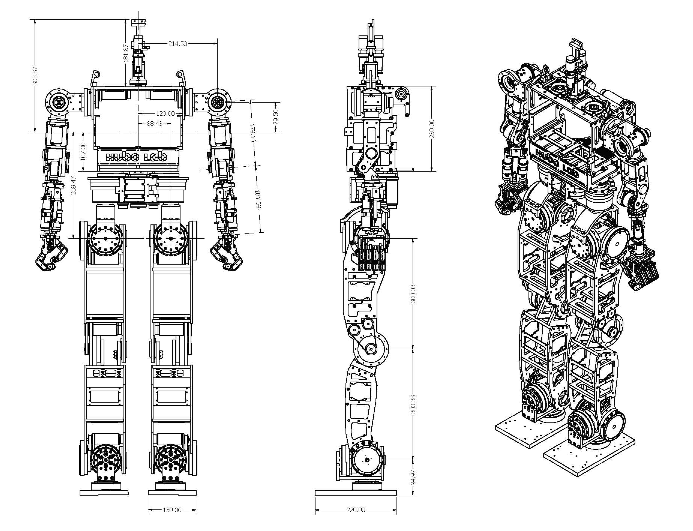
\includegraphics[width=1.0\columnwidth]{./pix/huboSch.png}
  \caption{Jaemi Hubo: 130cm tall 45kg (with battery and protective shell) 40 degree of freedom, high gain position controlled adult-size humanoid robot }
  \label{fig:huboSch}
\end{figure}



%We can never say that no parts will fail however we can know when they do and not have the entire system fail because of one part (reword).
%On April 27th, 2010: Jaemi Hubo was schedule to be apart of the \textit{Arts and Science Council} annual awards ceremony at the Philadelphia Convention Center.  During the dress rehearsal one of Jaemi's actuators failed ans she fell off of a 1.2 meter stage.






